\documentclass{article}
\setlength\parindent{0pt}
\usepackage[hmargin=1in,vmargin=1in]{geometry}
\setlength{\parskip}{.5em}
\usepackage{graphicx}

\title{CMPT 409 Assignment 6}
\author{Heather Li, Ekjot Singh Billing, Manshant Singh Kohli}

\begin{document}
\maketitle

\section{Bejeweled}
Completely Done
Bruteforce, at most (7*8)*2=112 swaps



\section{Binary}
Completely Done
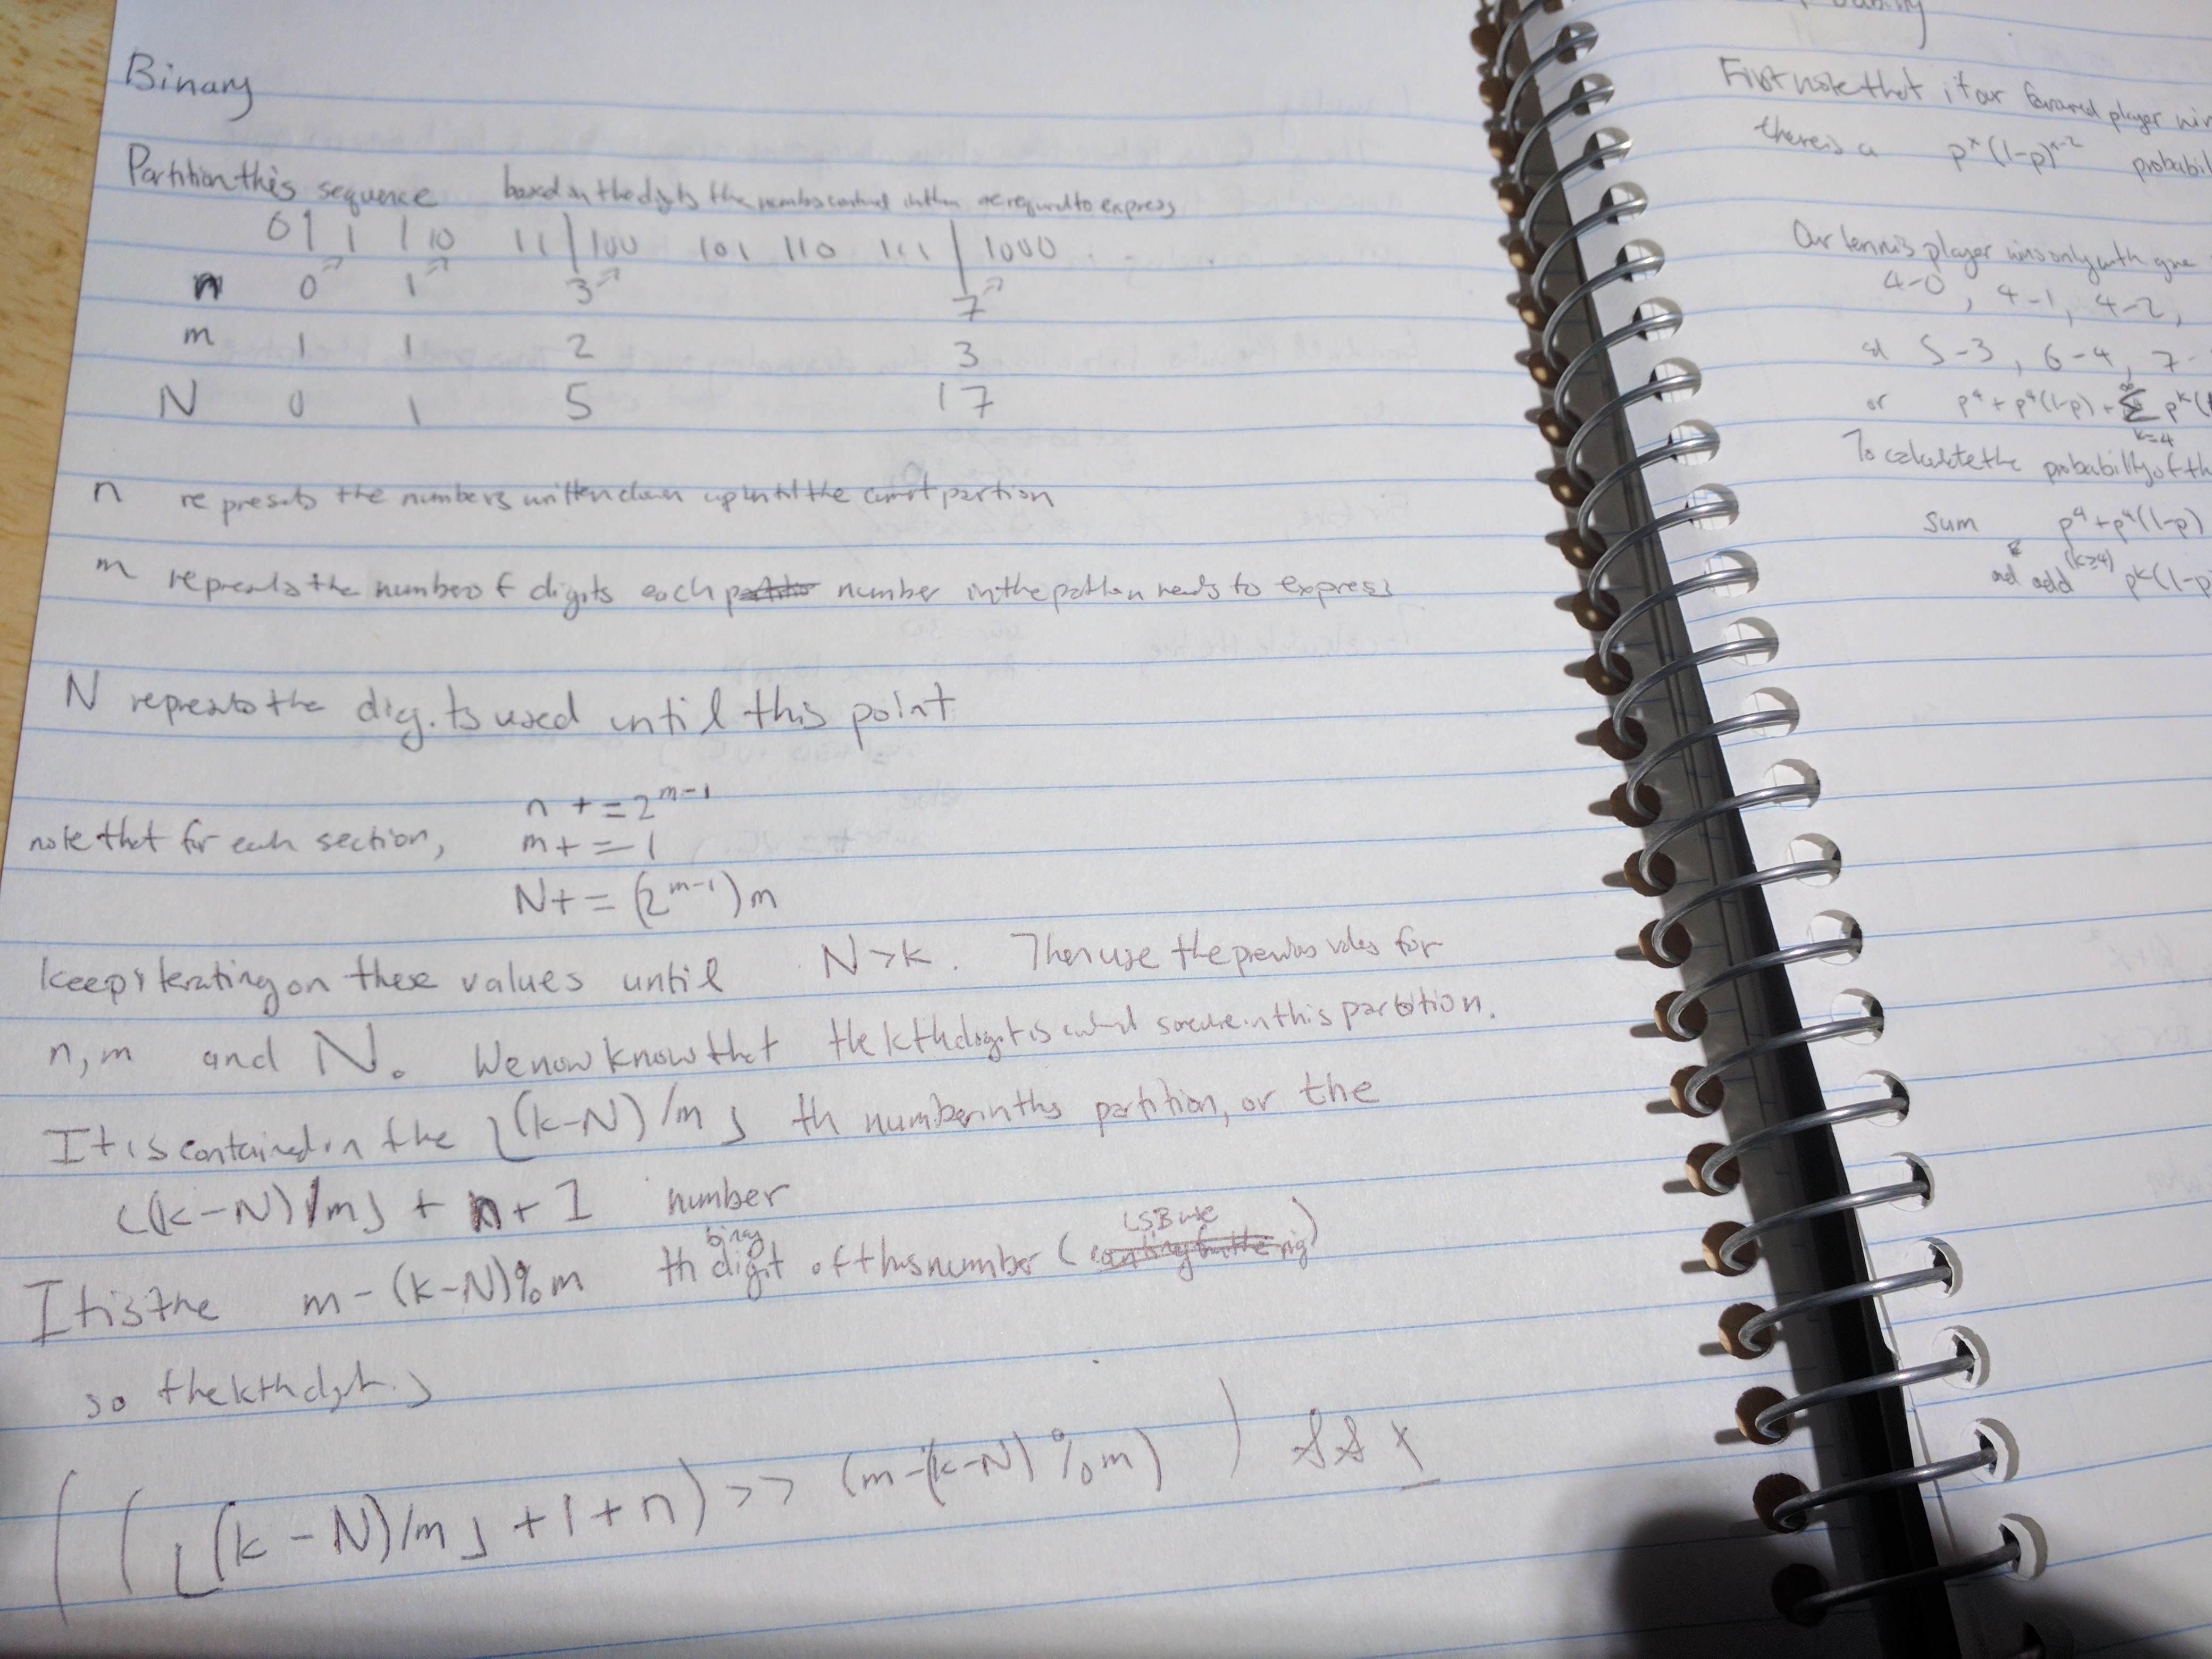
\includegraphics[width=.75\textwidth]{binary}

\section{City Slickers}
First, I do a graph coloring and create disjoint sets of '.' and 'r', and keep track of the 2 groups that contain the 'r's. If both the 'r's are in the same group then the answer is 0. This can be computed in O(r*c) time.
\par
Next, I create a graph where the edges are stored in HashMap where the key is the x,y coordinates and the value is a HashSet of all the edges it connects to. I am using this since it provides me a O(1) time add and query edges of a node. I then store all the surrounding mountains in (north, south, east, west) of each mountain with the joining mountain. This can be done in another O(r*c) time.
\par
Next, for each one of the colored groups above, I create an c++ vector of mountains surrounding that group. Then I create an edge from each mountain in the vector to every other mountain. This can be done in another O(r*c) time.
\par
Now All is left is a simple BFS graph treversal from one group with 'r' to another since the HashMap contains the edges for immediate reachable mountains and the minimum route represents the minimum number mountains that are needed to be crosed to reach the destination. For this we can do this iteratively by using a Queue, and a HashSet. Queue will contain the next coordinates to visit and the minimum number steps needed to get to these coordinates. HashSet will contain where mountain at this coordinates has been visited during the BFS treversal before or not. This BFS will take another O(r*c) time.
\par
So the total algorithm will take O(r*c) time

\section{Cutting Pizza}
Completely Done
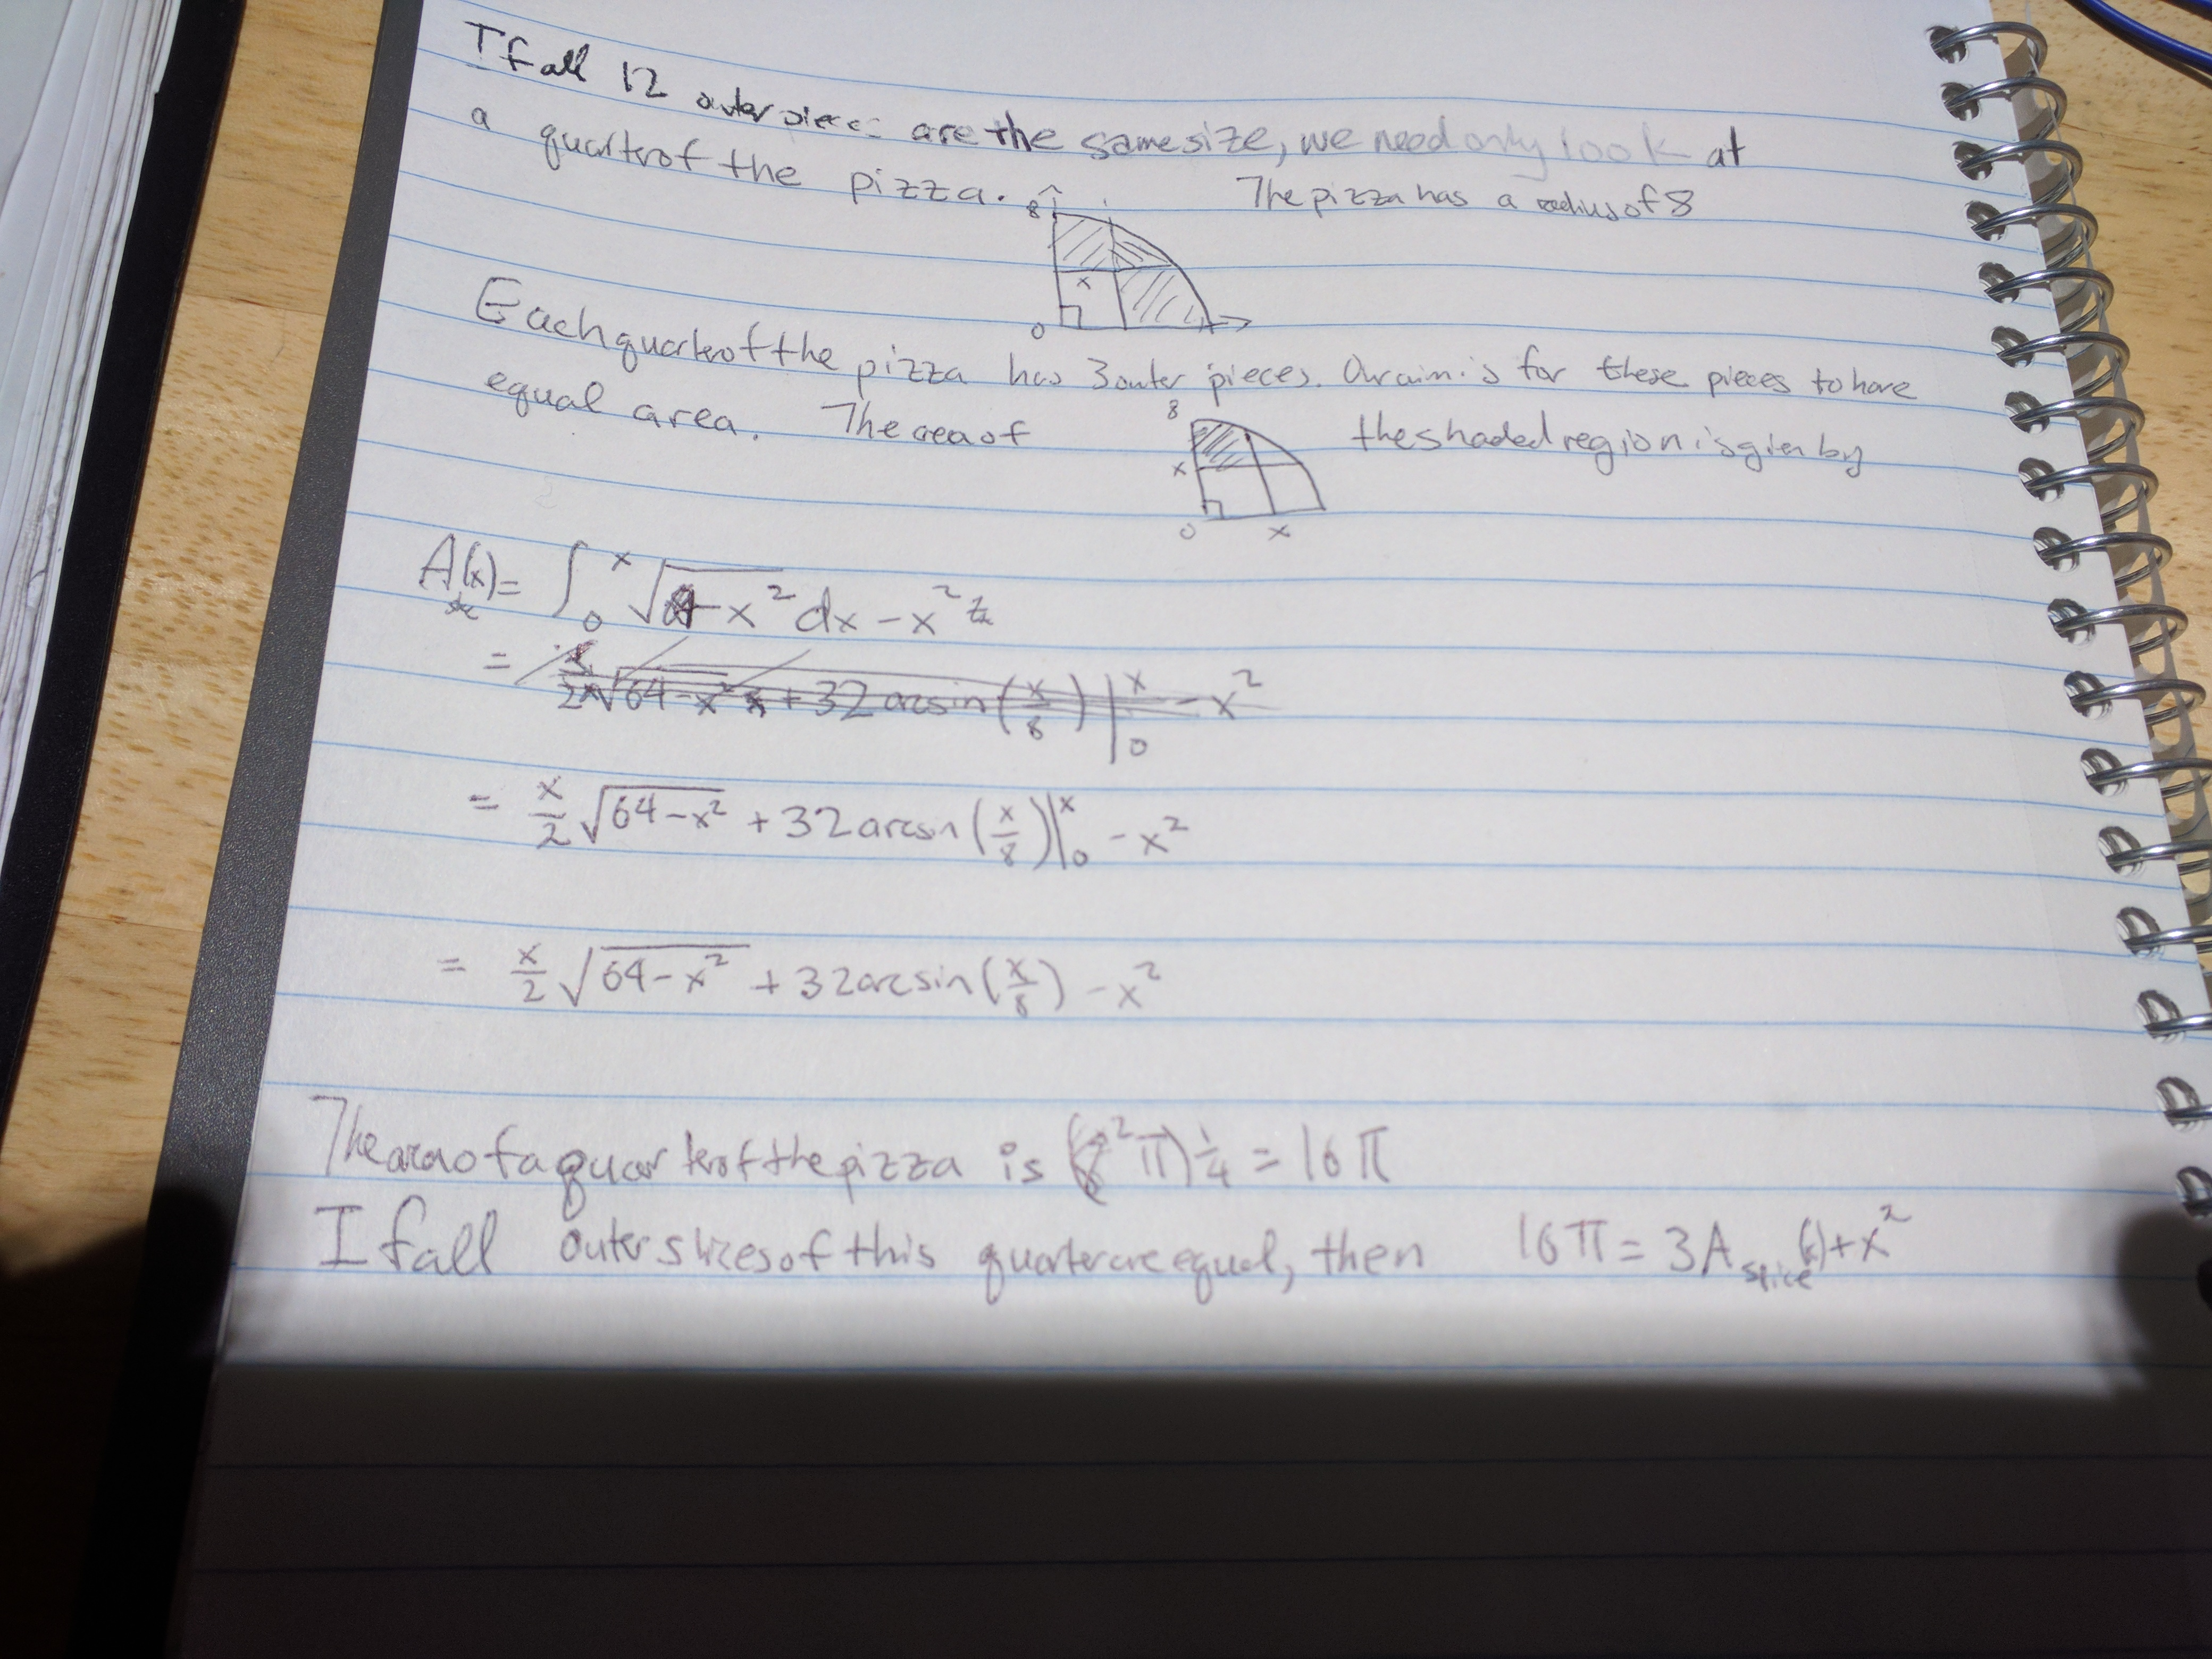
\includegraphics[width=.75\textwidth]{pizza}

\section{Doing Laundry}
Completely Done
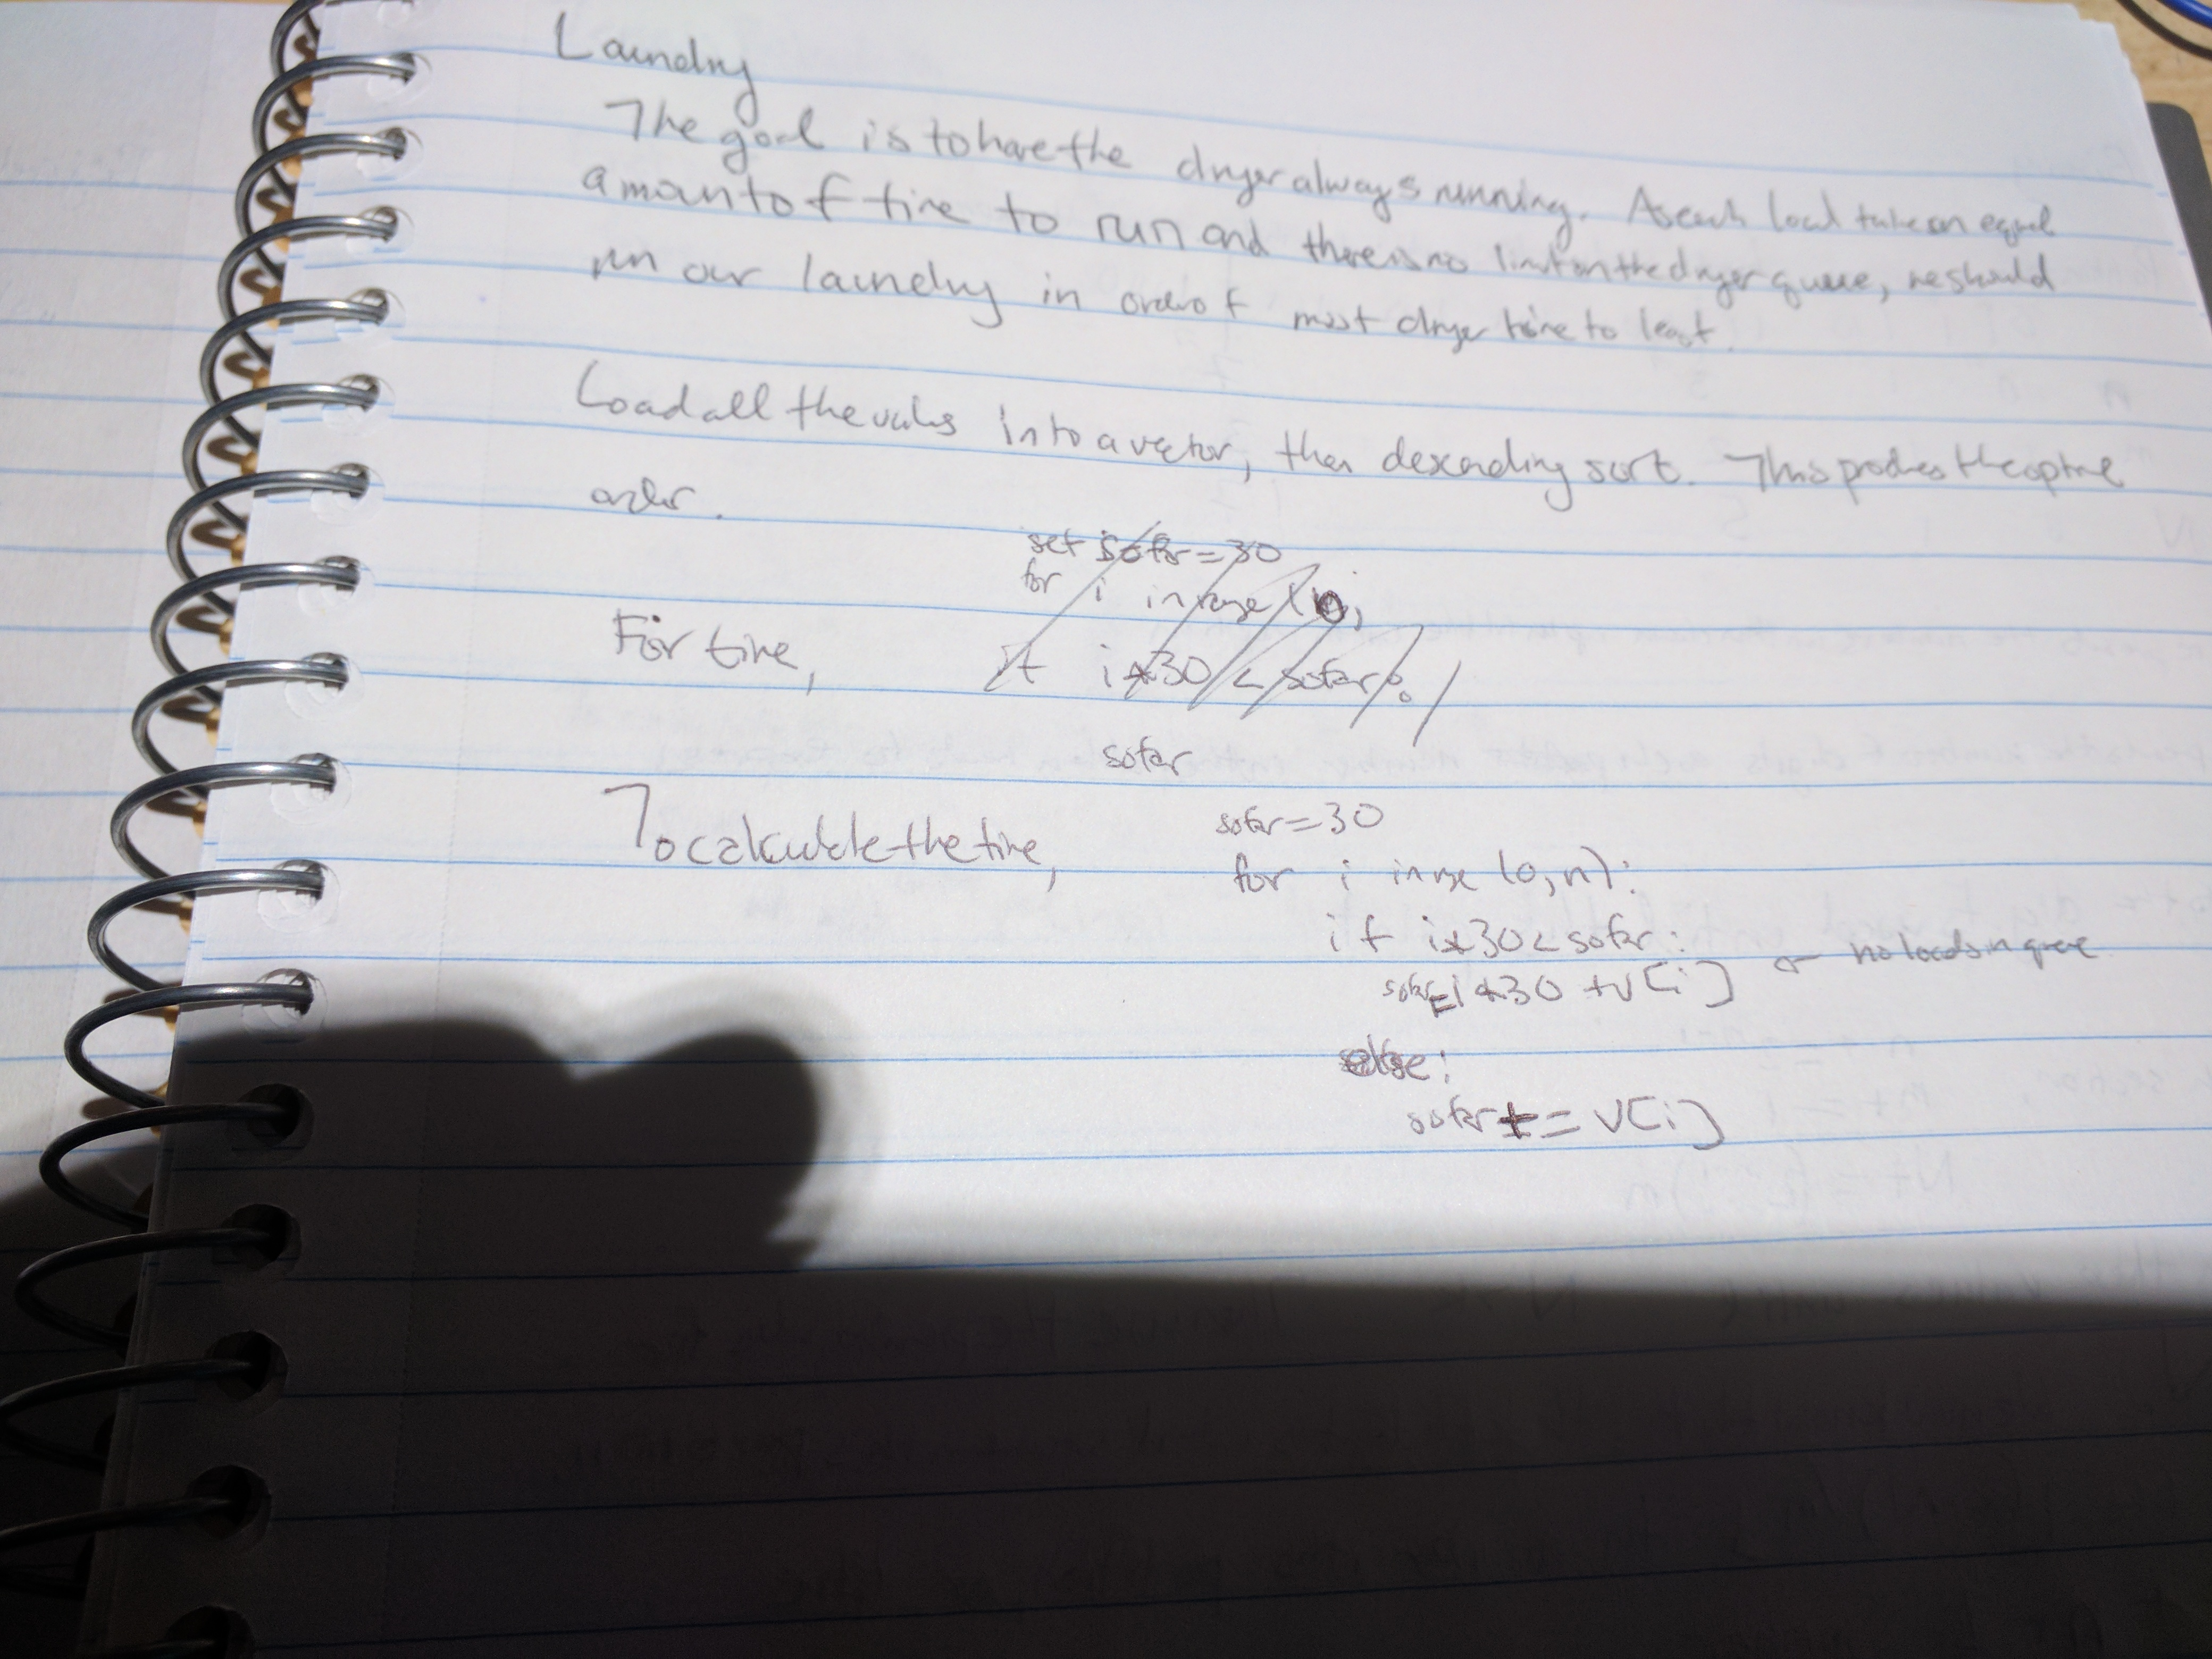
\includegraphics[width=.75\textwidth]{laundry}

\section{Linking Logos}
Kinda solution?

Partitions of n not hard to form. Create a bitmask of possible sums, with 1 where a break between two blocks would be. AND to see if there would be a disconnect. (needs pruning for time)

\section{Longshot}
Crappy solution, mostly done
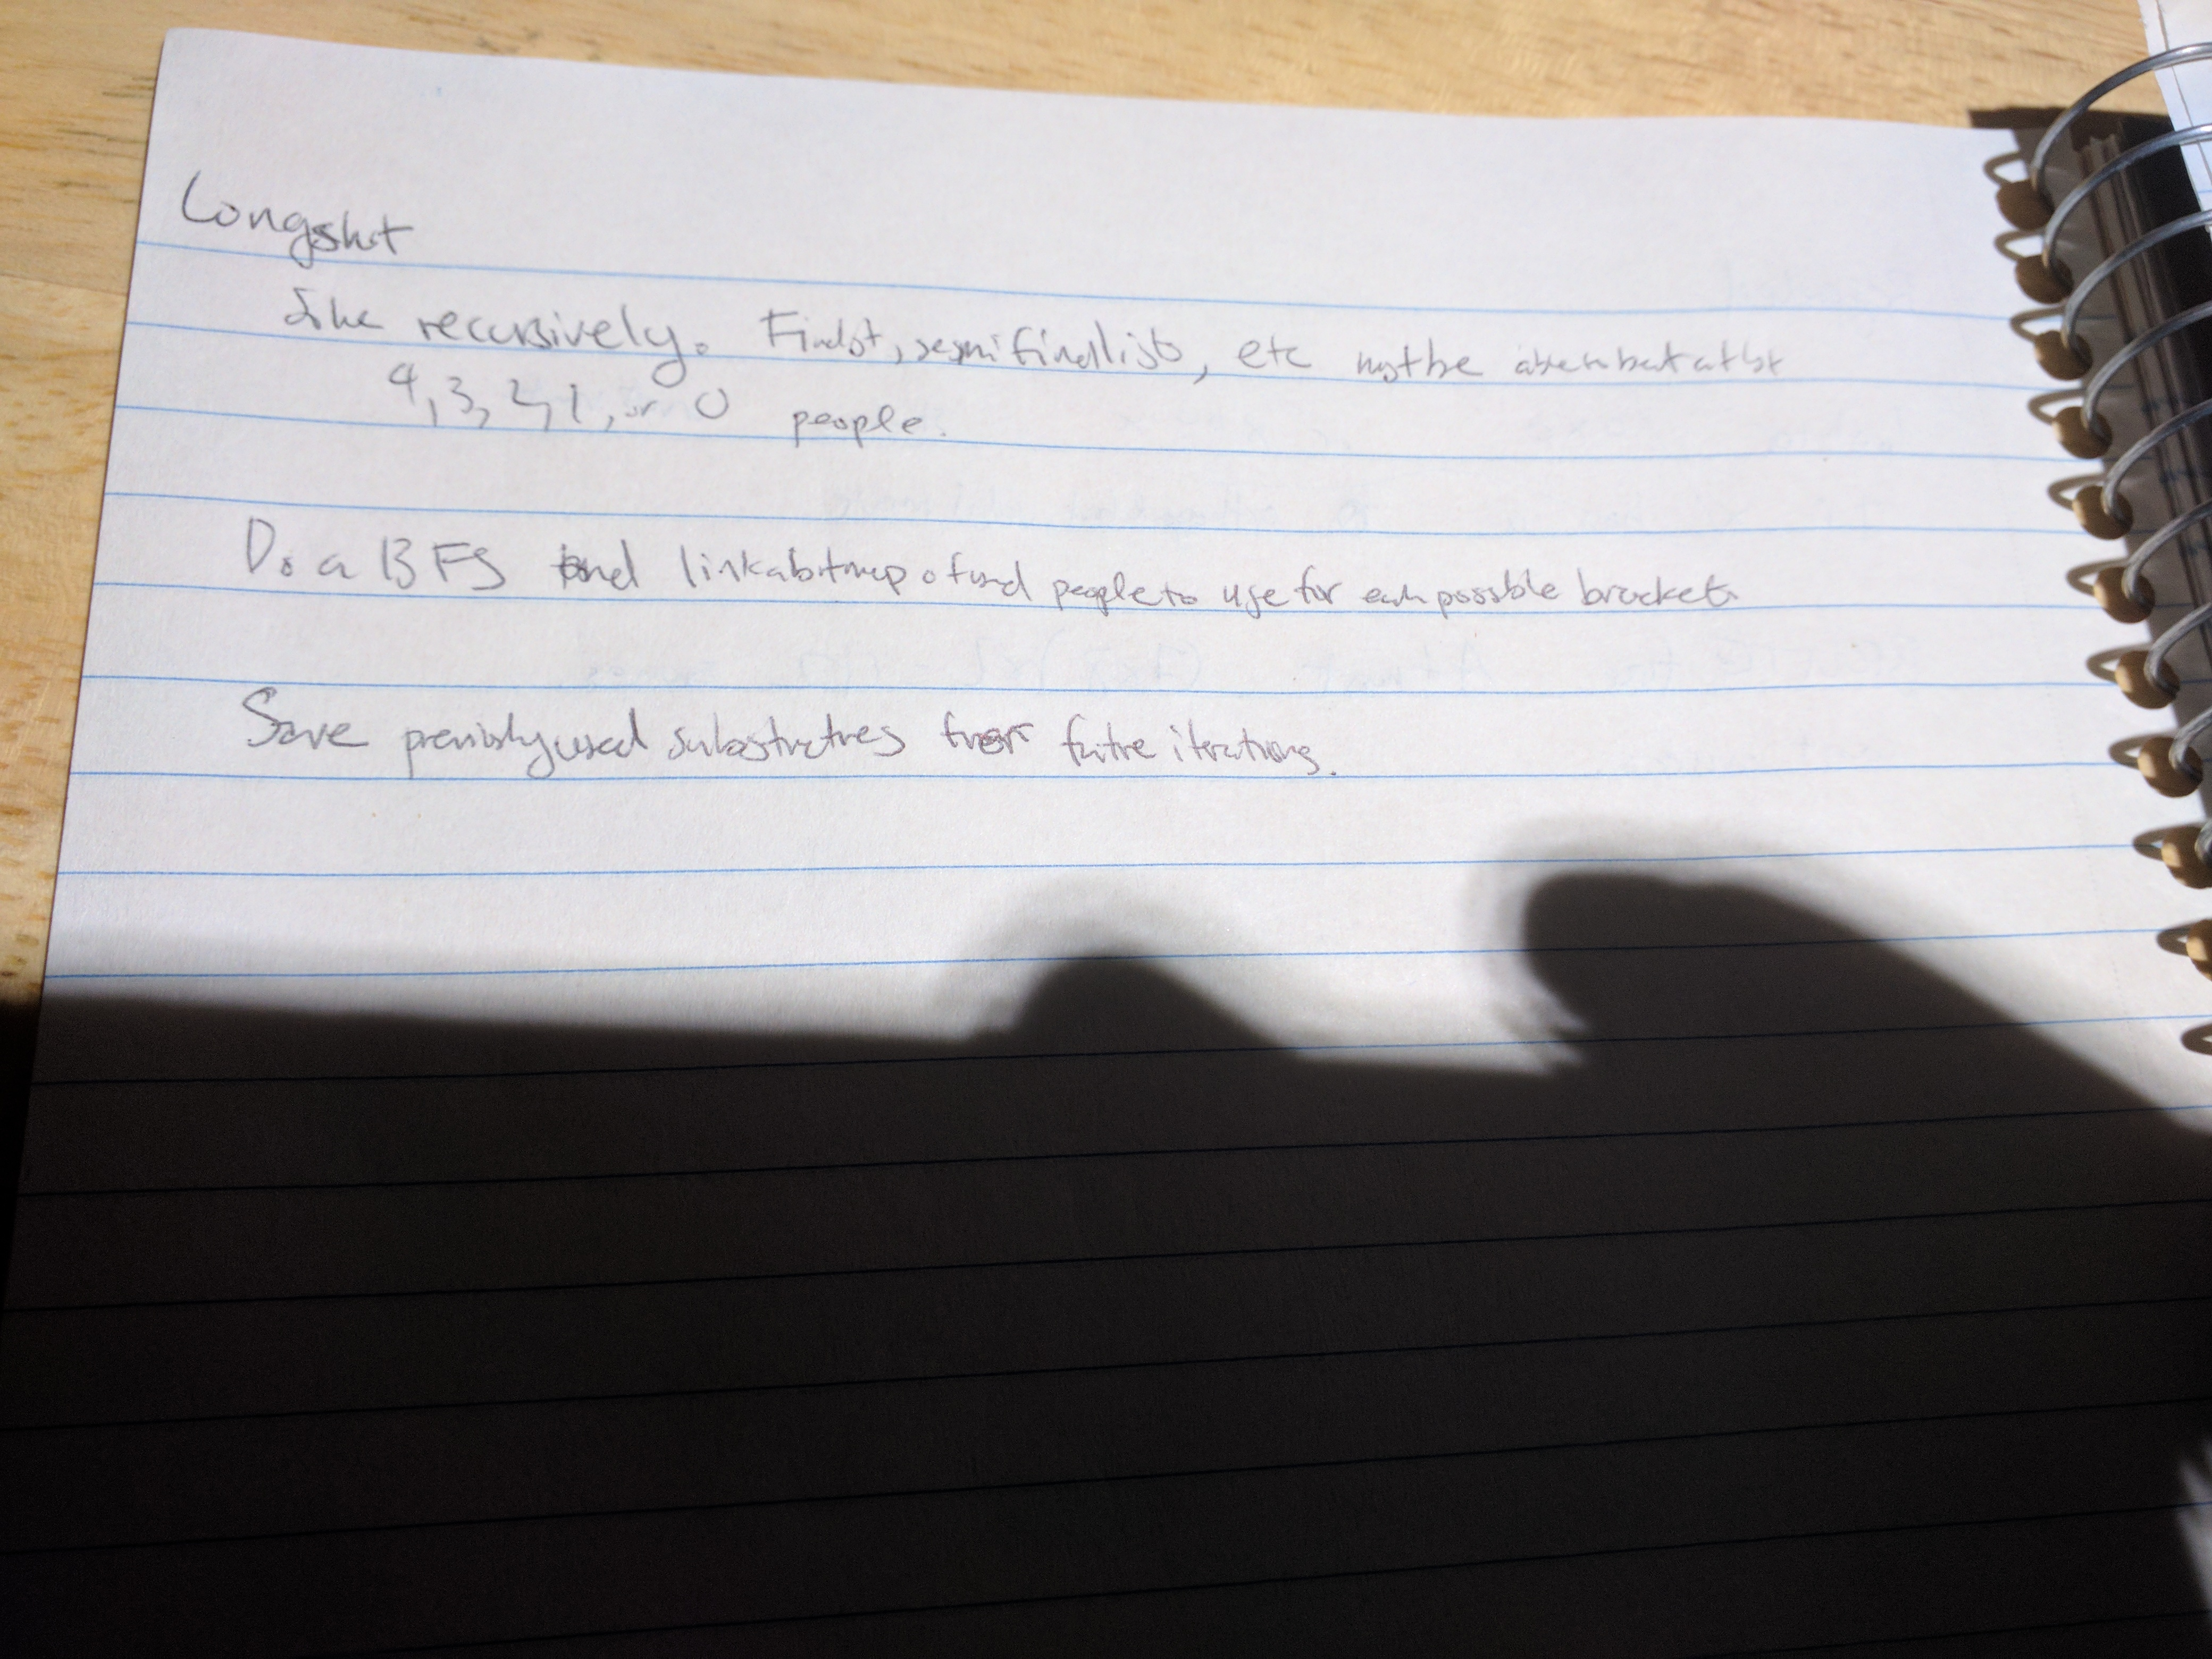
\includegraphics[width=.75\textwidth]{longshot}

\section{Prefix Goodness}
\noindent
Since we are only looking at the prefixes, we know that: for any 2 strings, if their prefix of size N do not match, then their prefix of size N+1 will not match as well. With this property, we can recursively find the best solution. Since we do not want to copy the string again and again, we only keep track of index. This can be done with a vector of size N which contains integers 1..N (representing the ith of the N strings).
Our recursive function \textbf{FIND\_SOLUTION} goes as follows:

\noindent
Function arguments:
\begin{itemize}
  \item \textbf{V}: The vector of string indexes
  \item \textbf{I}: The starting position of the current partition
  \item \textbf{L}: The length of the current partition
  \item \textbf{D}: Depth (can be thought of as index of the current characater to compare, or length of the current prefixes being compared - 1) in the current partition 
\end{itemize}

\noindent
Function body:
\begin{enumerate}
  \item If I $<$ 1, then return 0.
  \item If I == 1, then return D.
  \item We first perform a quick sort partion on the subarray V[I...I+L]. Based on the character at index D of each of the corresponding strings in the subarray. This gives us the indexes of the new partitions. \textbf{(Computed in O(L) time)}
  \item We recursily call this function \textbf{FIND\_SOLUTION} again on both the partitions and keep track of the maximum result given by these two partitions in a variable \textbf{tempMax}.
  \item we return the  max(tempMax, D*L).
\end{enumerate}

\noindent
The runtime of the algorithm depends on the in the input. In the very worst case partitioning, it would take O(N*M) where M is the maximum length of any string.

\section{Quantum Teleporters}
Shortest path problem from hell. Simple graph, but not a tree.


\section{Tennis Probability}
Completely Done
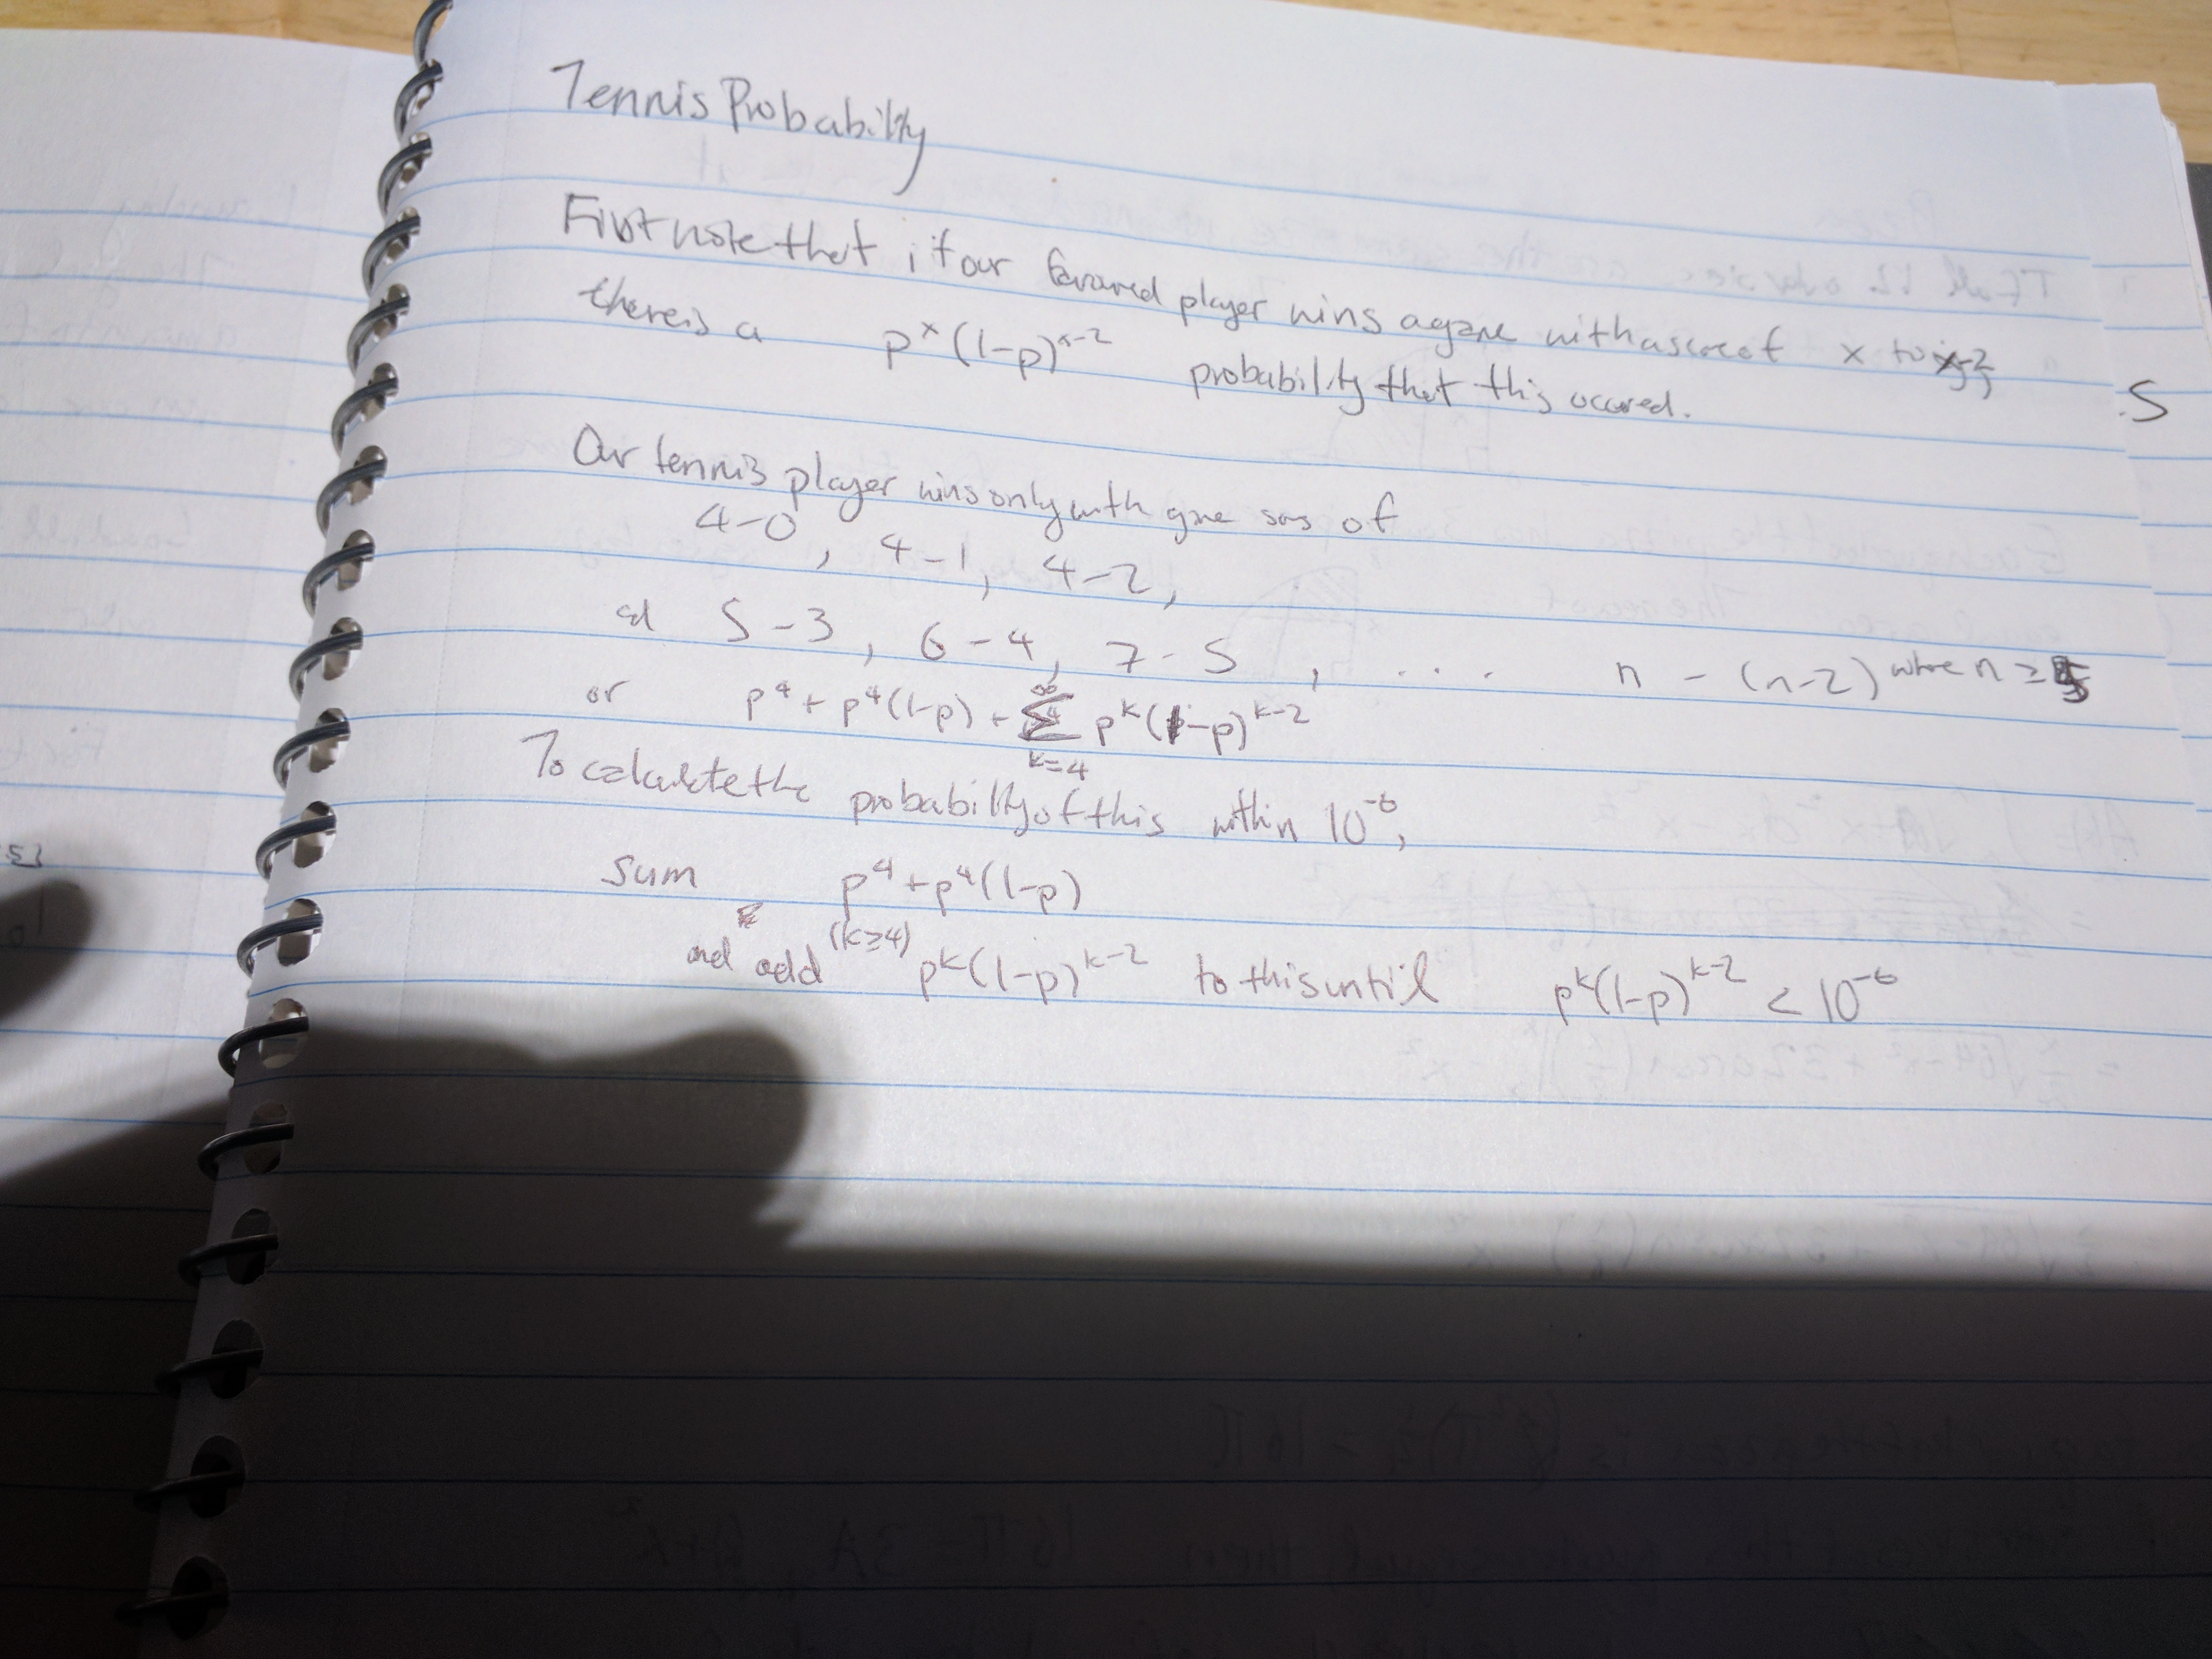
\includegraphics[width=.75\textwidth]{tennisprob}

\section{Zurch Trees}
Divide and conquer or something. Basically, the strategy is to leave an officer at stars and have an officer search the connected nodes. If this strategy is optimal, we just need some way of counting 'star depth'



\end{document}